%%
%% pytorch-neural-doodle/docs/content/chapters/03_results.tex
%%
%% Created by Paul Warkentin <paul@warkentin.email> on 21/08/2018.
%% Updated by Bastian Boll <mail@bbboll.com> on 07/10/2018.
%%

\section{Results}
\label{section:results}

We reproduced the results of \cite{doodles2016} by implementing the described algorithms on top of pytorch\footnote{The code for this implementation is publicly available at \url{https://github.com/paulwarkentin/pytorch-neural-doodle}. See the Readme for additional information.}. It is to be noted that style transfer using the approaches presented in the present work has at its heart an optimization procedure which is very demanding in terms of GPU memory and compute capability. The high memory requirements stem from the need to save and evaluate image patches. Fundamentally, the procedure takes time, because computing a gradient of the loss function requires a backward pass through the VGG network. Figure \ref{fig::phases} displays the progress of an L-BFGS optimizer for the generation of a stylized image.

\begin{figure}
	\begin{subfigure}[t]{0.23\textwidth}
		\centering
		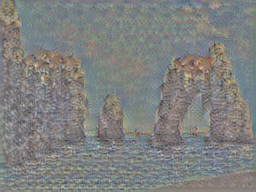
\includegraphics[width=3.5cm]{phases/output-50.png}
	\end{subfigure}%\hspace{5mm}
	~
	\begin{subfigure}[t]{0.23\textwidth}
		\centering
		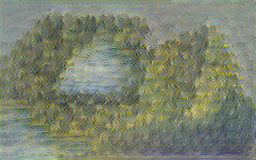
\includegraphics[width=3.5cm]{phases/output-200.png}
	\end{subfigure}%\hspace{5mm}
	~
	\begin{subfigure}[t]{0.23\textwidth}
		\centering
		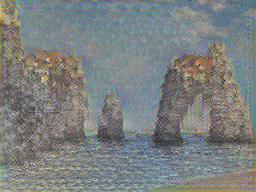
\includegraphics[width=3.5cm]{phases/output-400.png}
	\end{subfigure}
	~
	\begin{subfigure}[t]{0.23\textwidth}
		\centering
		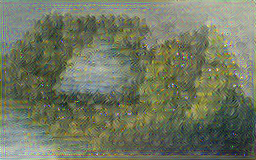
\includegraphics[width=3.5cm]{phases/result.png}
	\end{subfigure}
	
	\caption[]{Progress of an L-BFGS optimizer for the generation of a stylized image. Iteration count from left to right: 50, 200, 400, 500.}
	\label{fig::phases}
\end{figure}